\chapter{Methodology}

In this chapter we will go over the methods used to build and train our own pose estimation model.

\section{Fully Rendered Datasets}

\subsection{Motivations and Objective}

We find ourselves in the situation where we want to train a 6D pose estimation model on a set of objects that is not present in any available dataset. Therefore the first essential step to developing our model is the creation of our own datasets for training and evaluation.

These datasets consist of a collection of images containing the object we wish to track, with associated ground truths encoding the pose of the tracked object for each image. Collecting this data in the real world is tedious and difficult, considering the number of samples required for deep learning, and that any errors or biases will strongly affect the perfomance of the trained model. 

One possible solution is to use rendering software, which can generate potentially infinite quantites of training images with associated, perfectly accurate ground truths. However, while a model trained on this data could function in simulation, we have no guarantee whether it would also function in real life. This is because a simulated sensor and simulated enviroment are unable to reproduce unmodeled physical effects and noise in the same way a real sensor would with a real environment. This issue, dubbed the "reality gap"\cite{domainRandomization2}, is recurring in any field which relies on simulations to supply data.

Domain Randomization\cite{domainRandomization} is one of the most utilised methods for solving this issue. It states that introducing sufficient variability in the simulated domain will allow the model to generalise to the real world with no additional training. This allows us to entirely skip the laborious data collection step and instead rely on a 3D model of the object we wish to track, which is usually readily available and accurate.

\subsection{Generation Methodology}
\label{ss:ScrewDataset}

To render the images for our dataset, we used the Unity Perception package\cite{unityPerception}, which integrates domain randomization features into its pipeline. Unity Perception works by simulating a scene, and then rendering each simulated frame from the perspective of a virtual camera. 

When setting up the simulation, we specify the number of iterations to simulate and the number of frames to render for each iteration. At the beginning of each iteration, we call a set of randomizers; each randomizer is a script that sets one of the domain variables for the iteration, such as the pose of an object or the colour of the light source. The scene is then updated according to the domain variables, rendered, and the associated ground truth saved.

\begin{figure}
    \centering
    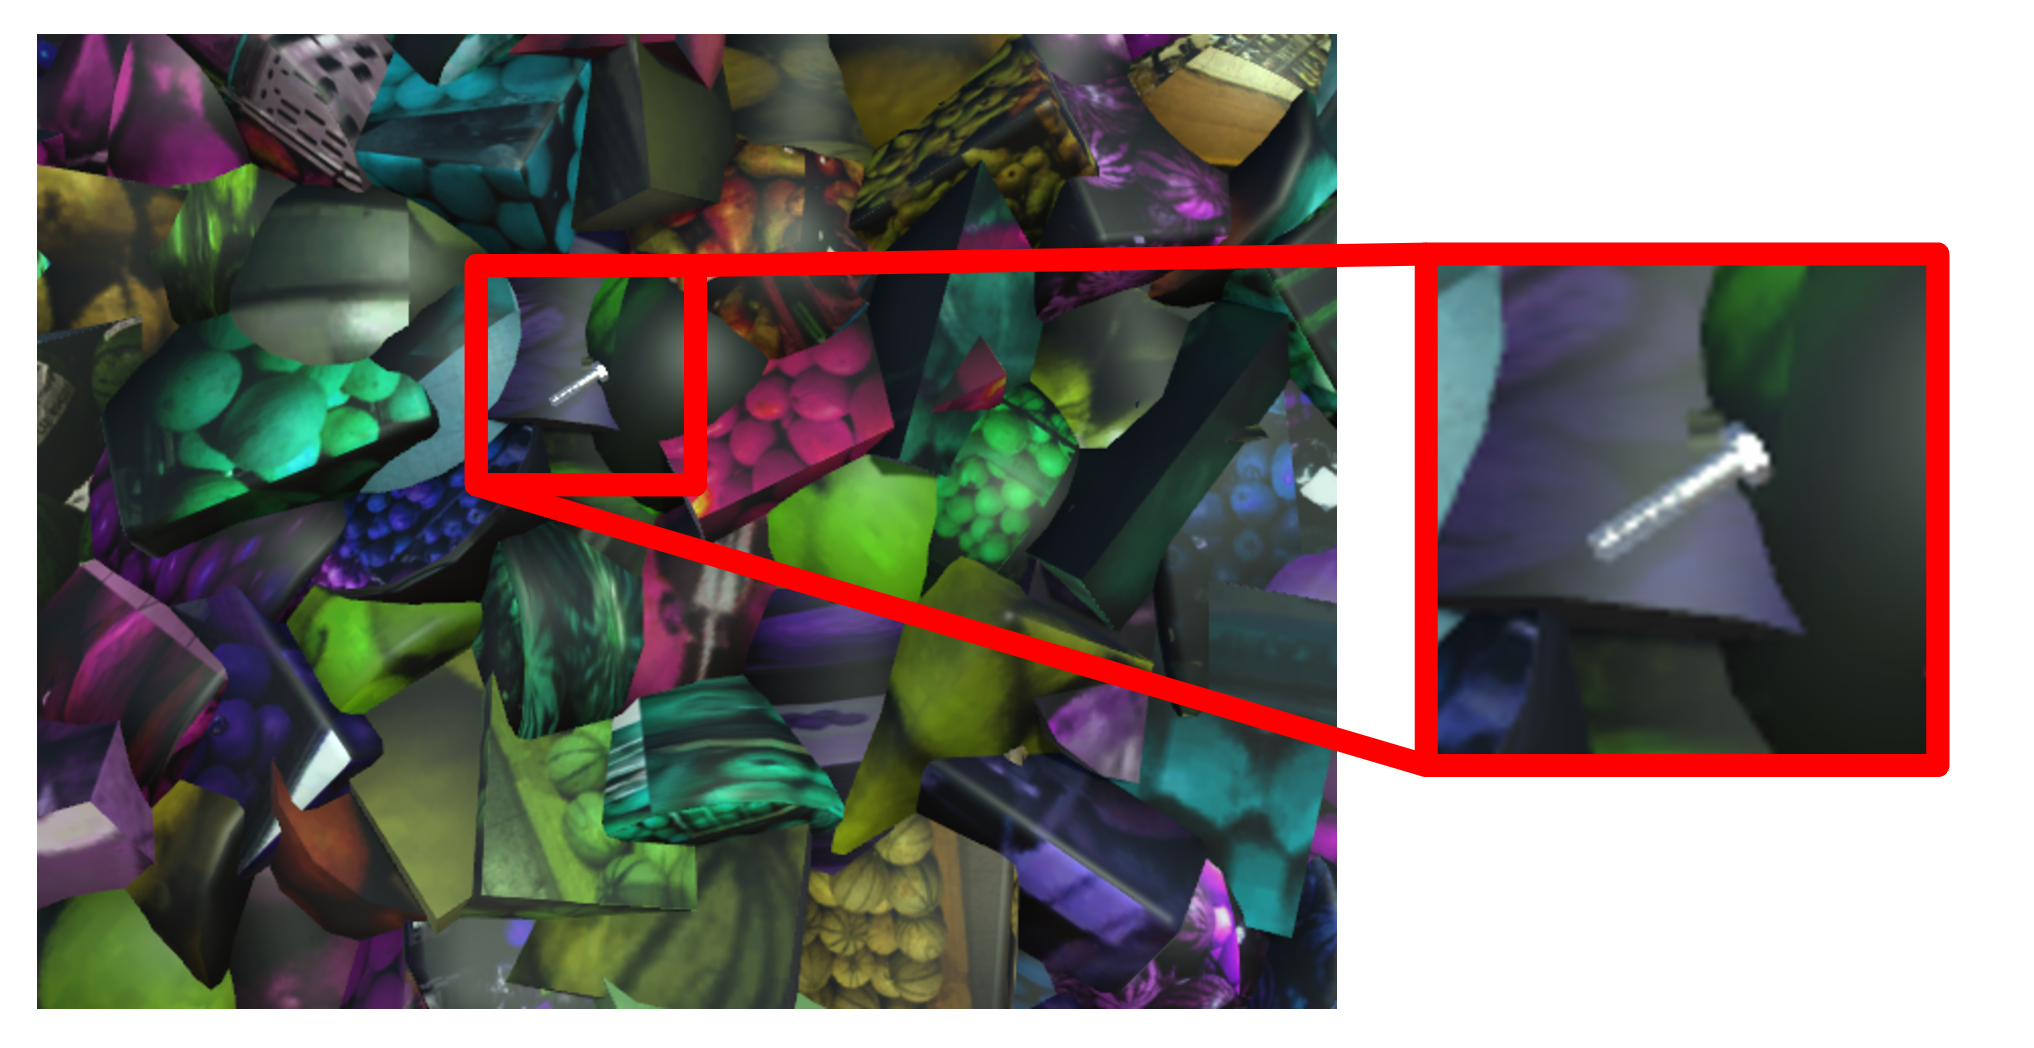
\includegraphics[width=0.6\textwidth]{screwdataset/ScrewDataset.png}
    \caption{One of the images generated with Unity's Perception package for training our model, with a zoom-in on the screw.}
    \label{fig:screwdataset}
\end{figure}

As a test case, we decided to generate a pose estimation dataset for a standard M6x30 hexagonal head screw. This is a very challenging object, as it is small and symmetric. The reason why symmetric objects are difficult for pose estimation is explained in depth in appendix A.2. The model of the M6x30 screw was obtained from the FreeCAD Fasteners workbench\cite{Fasteners} and colored with a metallic texture.

The domain for this dataset consists of images of the screw placed inside of a scene: thus the primary domain variables are the pose, the background, and the lighting. We used a custom randomizer to set position and rotation for each iteration, and default randomizers provided as part of the Perception package to generate a background, composed by random 3D shapes placed with random positions, orientations and textures. Finally, we used a custom randomizer to set the lighting color, intensity and origin. A sample image from this dataset appears in figure \ref{fig:screwdataset}.

We can then interface the output of this procedure with EfficientPose using a conversion script, which performs the necessary tasks to make the dataset compatible with the generators used by the network. In this manner we can quickly and easily generate arbitrarily large datasets for training, by first running the Unity scenario, and then running the conversion script for EfficientPose.

\subsection{Training}

The original version of EfficientPose is trained on LINEMOD. However, the specifics of LINEMOD and of our own dataset are widely different: LINEMOD has around 1200 images per object, and only about 200 of these are used for training, while our dataset has 10000 images, 9000 of which are used for training. This means that we must set proper training parameters for our own situation.

First, we reduced the number of epochs from 5000 to 100. Since our dataset contains 45 times more images, these two values represent a similar training time. EfficientPose also by default evaluates the model only every 10 epochs due to the small epoch size; we change this value to evaluate at the end of every epoch.

EfficientPose implements Keras' ReduceLRonPlateau callback to dynamically set the learning rate during training. This is standard practice: large learning rates quickly adjust the model but can lead to fluctuations, local minima and divergence; smaller learning rates avoid these issues but take an excessive amount of time to improve the model\cite{ReduceLR}. This method instead starts with a large learning rate, and then automatically reduces the learning rate whenever training stagnates, thus maintaining a value closer to the ideal. By default, EfficientPose halves the LR every time the accuracy does not improve for 25 epochs; we changed this to an 80\% reduction every 5 epochs, to account for the increased number of samples per epoch. The beneficial results of this process are visible in figure \ref{fig:screwdataset_training}: after epoch 27 the sudden drop in training and evaluation loss is due to a reduction in learning rate.

The initial and minimum learning rates are mantained identical to EfficientPose's, set at $10^{-4}$ and $10^{-7}$ respectively.

\subsection{Results}

\begin{figure}[ht]
    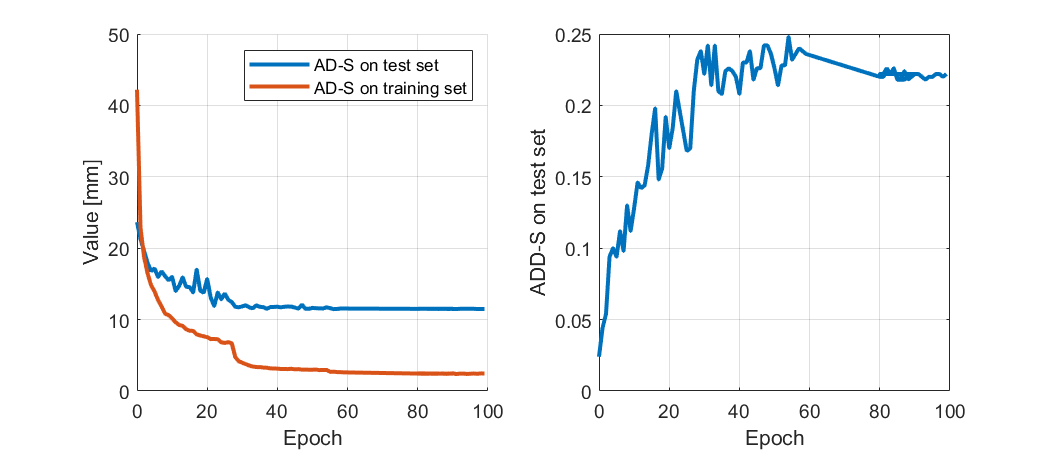
\includegraphics[width=\textwidth]{screwdataset_training.png}
    \caption{Evolution of the loss, AD-S and ADD-S metrics during training. The loss in this case is computed as the AD-S metric on the training dataset.}
    \label{fig:screwdataset_training}
\end{figure}

After 100 epochs of training, the progress of which is shown in figure \ref{fig:screwdataset_training}, the model has a final ADD of 22.2\%, with a peak value obtained during training of 24.8\%, much lower than the 97.35\% reported on LINEMOD. We can hypothesize that the reason for this performance gap is that the rendered dataset is much more difficult than LINEMOD, since we are dealing with a very small, symmetric object hidden inside a chaotic, colorful background with widely differing light conditions.

Another serious issue, that is more difficult to convey on paper, is that the model is not able to bridge the reality gap: while testing in real-life scenarios, it failed to identify the screw in most conditions, let alone produce accurate estimations. This means that it generalises poorly outside of the simulated environment, making it essentially unuseable.

\section{Partially Rendered Datasets}

\subsection{Motivations and Objective}

As stated above, the model trained on our custom dataset has very poor performance, both in simulated scenarios and in real-life applications. Since the same model has no similar issues when trained on LINEMOD, we can hypothesize that the cause lies with the training dataset itself, for two reasons:

\begin{enumerate}
    \item The training images are too difficult compared to the task we want to perform, preventing the network from learning properly.
    \item The training images and the real-life captures are excessively different, thus the model is not able to bridge the reality gap.
\end{enumerate}

The second issue is the most debilitating, as it makes whatever model we train completely unapplicable to any real life situation. We hypothesize that, since the backgrounds we generated are composed of a compact assortment of random shapes, with random sizes, colors, texures and poses, the resulting dataset is adeguate for representing extremely cluttered and noisy environments, but inadeguate for most other environments.

We have two options for facing this issue. The first would be to make the backgrounds more general in scope. This could mean, for example, generating a wider variety of synthetic backgrounds, or alternatively using sets of photographs, such as the COCO or Imagenet datasets, as other approaches have already done\cite{DPOD}. This would allow the model to generalise to more situations, including eventually our usecase. This is probably the best option if we forsee a wide application of the model in a variety of different conditions, for example in an autonomous driving scenario.

The second option is to generate a set of training images that more accurately depict a small number of chosen environments. This makes it easier for the model to bridge the reality gap by making this gap "smaller", reducing the differences between the training dataset and the typical image seen during inferencing. However, we have fewer guarantees on performance outside of the selected environments, which makes this approach better for usecases which are stationary or limited to fewer settings. This is often the case for industrial applications, making this second option our preferred choice.

Thus our objective is to create a method to easily and quickly generate a realistic training dataset for our testing environment, which is a simple table with the objects placed on its surface.

\subsection{Generation Methodology}

We again use Unity Perception to generate our training dataset, as described in \ref{ss:ScrewDataset}. We used models for 5 objects: the same M6x30 screw used previously, a M8x16 round head screw, a M8x25 and M8x50 socket head screws, and a M4x40 countersunk screw. As previously stated, these are small, symmetric objects that are generally challenging to identify, with the additional complication that they all have similar shapes and sizes. Only the first four  are annotated, while the M4x40 is included as a "decoy" to reduce the number of false positives.

The key issue now becomes the positioning of the objects in the image. Since in real-life conditions, the pose of an item is almost always influenced to some degree by its environment, we believe that simply placing the item freely in 6D space as we did in the previous approach would lose information compared to a realistic placement. Taking our example setting where the objects are placed on a surface, this constrains three degrees of freedom for each object: the vertical position relative to the surface, and the two rotations around the axises that determine the surface itself. Thus our objective is, for each image, to start from the pose of the surface relative to the camera, and from there generate a realistic pose for each dataset object, so that the object appears to be placed on the surface.

We thus captured a video of the testing table, which had been prepared with an ArUco marker in its centre. After eliminating blurry and off-center frames, we undistorted the images to obtain the set of backgrounds. Undistorting is an important step: it reduces the reality gap between the virtual sensor with no distortion and the real camera. To reduce it further, we set up the virtual sensor so that it imitates the parameters of the camera itself, an Azure Kinect sensor with a 1280x720 resolution and 90\degree field of view.

Once we have a set of background images, the placement surface in each image will be highlighted by an ArUco marker, thus we can easily obtain the position and rotation of this surface, as previously described in section \ref*{s:notlearningbasedmethods}. This results in a reference system corresponding to the marker, determined by a translation vector $t_s$ and a rotation matrix $\text{R}_s$, expressed relative to the camera reference system.

We then want to place the object's model with a random position and orientation on this surface. To do this, we can consider its pose relative to the marker reference system, which is given by a translation vector $t_r$ and a rotation matrix $\text{R}_r$. We can compute values of $t_r$ and $\text{R}_r$ considering the constraints of the surface:

\begin{equation}
    t_r = 
    \begin{bmatrix}
        x_r\\y_r\\0
    \end{bmatrix}
    ,\; \; \text{R}_r =
    \begin{bmatrix}
        \cos \theta_r & - \sin \theta_r & 0 \\
        \sin \theta_r & cos \theta_r & 0 \\
        0 & 0 & 1
    \end{bmatrix}
    \label{eq:translationsurface}
\end{equation}

... where $x_r$, $y_r$, and  $\theta_r$ are our three remaining free variables. We can extract their values from pre-defined probability distributions; in our case we used three uniform distributions $U(x_{min}$, $x_{max})$, $U(y_{min}, y_{max})$, and $U(\theta_{min}, \theta_{max})$. Essentially, \ref{eq:translationsurface} means that each object is free to translate along the surface, and to rotate around the axis perpendicular to the surface. Thus we can compute its pose $(t, \text{R})$ in the camera reference as:

\begin{align}
    t &= t_s + \text{R}_s t_r \label{eq:wrongpostionequation} \\
    \text{R} &= \text{R}_s \text{R}_r \nonumber
\end{align}

However, this operation alone is flawed, as it would place the origin of the 3D model on the surface, but for the objects in our dataset, the model origin is in the centre of the object. Therefore we must implement a final roto-translation that places the object on the surface starting from the position computed in \ref*{eq:wrongpostionequation}. This transformation differs based on the object, for example, if we consider the M6x30 screw, this correction transformation $(t_c, \text{R}_c)$ is given by a translation $z_c$ along the z-axis and a rotation by $\theta_c$ around the y-axis:

\begin{equation*}
    t_c = 
    \begin{bmatrix}
        0\\0\\z_c
    \end{bmatrix}
    ,\; \; \text{R}_c =
    \begin{bmatrix}
        \cos \theta_c & 0 & -\sin \theta_c\\
        0 & 1 & 0\\
        \sin \theta_c & 0 &  \cos \theta_c
    \end{bmatrix}
\end{equation*}

...where $z_c$ and $\theta_c$ depend on the dimensions of the screw as follows:

\begin{align*}
    \theta_c &= \frac{\pi}{2} - \arctan \frac{l_2}{l_1}\\
    z_c &= \frac{1}{2}d \sin \theta_c + \frac{1}{2} l \cos \theta_c
\end{align*}

The final pose in camera reference is then given by:

\begin{align*}
    t &= t_s + \text{R}_s t_r + \text{R}_s \text{R}_r t_c\\
    \text{R} &= \text{R}_s \text{R}_r \text{R}_c
\end{align*}

One thing to note is that if an object can have multiple positions on the surface, we consequently have multiple correction transformations to choose from. For example, each screw could be on its side or on its head, which implies a choice between two sets of $t_c$, $R_c$.

We implemented this method with Unity, using a custom randomizer that sets the pose of each object starting from the pose of the ArUco marker, which is pre-computed for each background image. We then have two more randomizers that set the background for each image and light intensity and rotation. A sample image from the final dataset is represented in figure TBA.

\subsection{Training}

The training dataset we generated has two major weaknesses. First, there is a limited number of background images, which means that the model has a finite number of camera positions to learn from, which in turn may lead to overfitting and unreliable results for positions that don't have sufficient representation. Second, it is difficult to randomize light intensity and color for the background images inside Unity, as it is decoupled from the same settings for the 3D models.

We can remedy these issues using data augmentation. This is a technique that involves applying random changes to data during training, similarly to how domain randomization would randomize them during generation. EfficientPose already provides two data augmentation methods: 6DoF and color. 6 Degree-of-Freedom augmentation involves randomly rescaling and rotating the input image and consequently adjusting the ground truth, so as to greatly increase the number of possible poses each image can provide. Color augumentation instead implements RandAugment\cite{RandAugment} to change the color and grain for the entire image. Applying both these methods results in images such as the one depicted in figure \ref{fig:ScrewPoseAugmented}, conveniently fixing the issues of our dataset.

Other training parameters are identical to the previous attempt with the fully generated dataset: 100 epochs, with an 80\% learning rate reduction if the model stagnates for 5 epochs.

\begin{figure}
    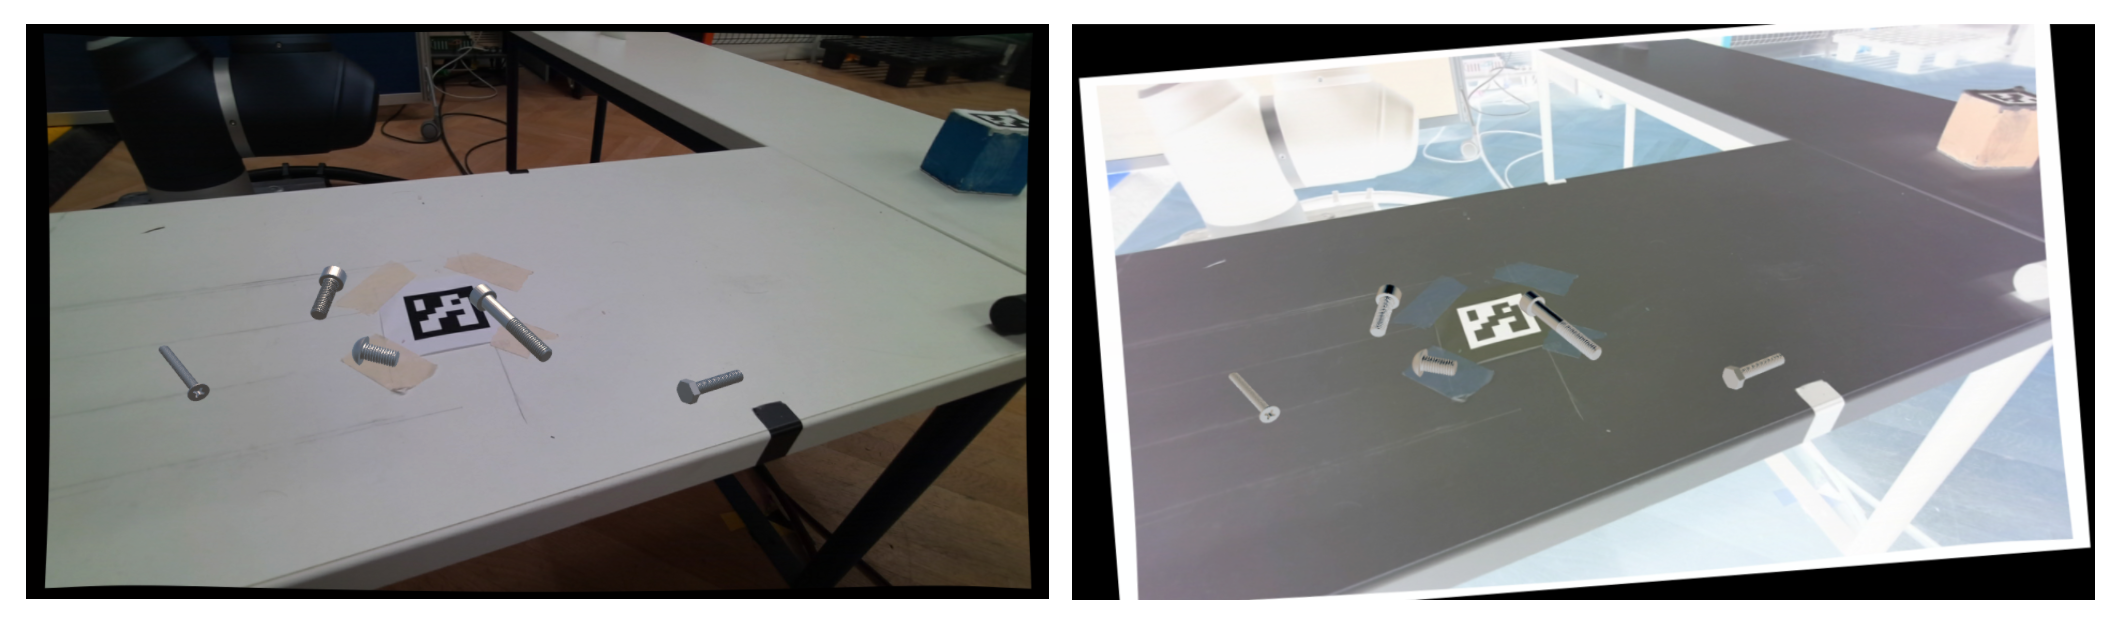
\includegraphics[width=0.7\textwidth]{screwposeaugmented.png}
    \caption{An example of a final training image resulting from data augmentation.}
    \label{fig:ScrewPoseAugmented}
\end{figure}

\subsection{Results}

\section{Semantics Applications}

\subsection{Motivations and Objective}

In many applications, it may be that estimating the pose of an object is sufficient to perform the task. However, in many situations it may be necessary to infer additional information from this data. An example may be the assembly of a workpiece from its components, where while tracking the pose of each individual component we may also have to track the state of the assembly itself.